\section{Precision-Recall and ROC curves}
\begin{multicols}{2}

\subsection{Precision-Recall Curves}

Precision-Recall Curves are very widely used evaluation method from machine learning. 

As we just saw in example, the x axis shows precision and the y axis shows recall. 

Now an ideal classifier would be able to achieve perfect precision of 1.0 and perfect recall of 1.0. So the optimal point would be up here in the top right. And in general, with precision recall curves, the closer in some sense, the curve is to the top right corner, the more preferable it is, the more beneficial the tradeoff it gives between precision and recall. And we saw some examples already of how there is a tradeoff between those two quantities, between precision and recall, with many classifiers. 


\begin{center}
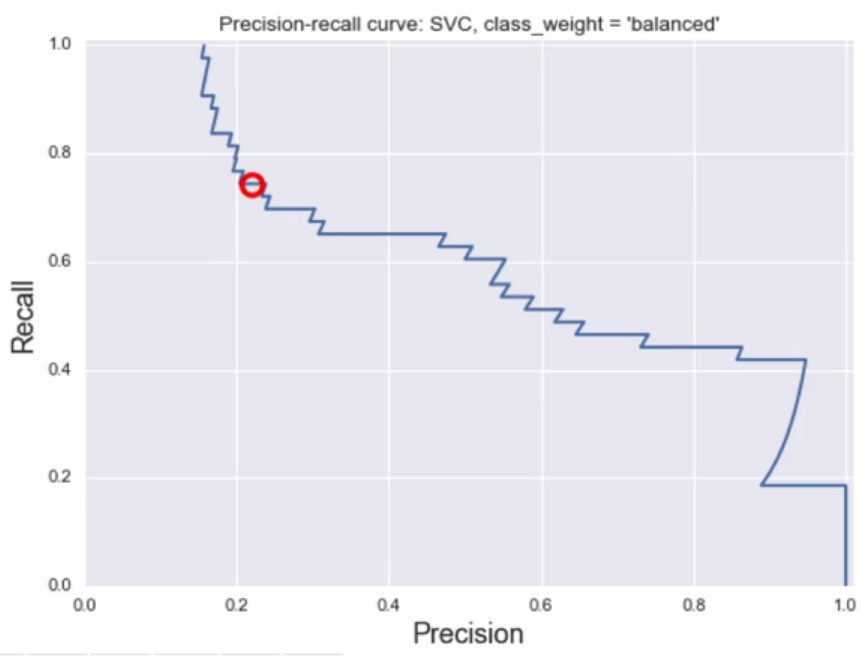
\includegraphics[width=\linewidth]{img/Precision-Recall-curve.png} 
\end{center}

This example here is an actual precision recall curve that we generated using the following notebook code. 

{\scriptsize
\begin{verbatim}
from sklearn.metrics import precision_recall_curve

precision, recall, thresholds = 
    precision_recall_curve(y_test, y_scores_lr)
closest_zero = np.argmin(np.abs(thresholds))
closest_zero_p = precision[closest_zero]
closest_zero_r = recall[closest_zero]

plt.figure()
plt.xlim([0.0, 1.01])
plt.ylim([0.0, 1.01])
plt.plot(precision, recall, label='Precision-Recall Curve')
plt.plot(closest_zero_p, closest_zero_r, 'o', 
    markersize = 12, fillstyle = 'none', c='r', mew=3)
plt.xlabel('Precision', fontsize=16)
plt.ylabel('Recall', fontsize=16)
plt.axes().set_aspect('equal')
plt.show()
\end{verbatim}
}
The red circle indicates the precision and recall that's achieved when the decision threshold is zero. So I created this curve using exactly the same method as we saw in the previous example, by looking at the decision function output from a support vector classifier. Applying varying  decision boundary, looking at how the precision of recall change as the decision boundary changed. Fortunately, scikit-learn has a function that's built in that does all of that, that can compute the precision- recall curve. 

So you can see that in this particular application there is a general downward trend. So as the precision of the classifier goes up, the recall tends to go down. 

In this particular case you'll see also that it's not exactly a smooth curve. There are some jaggy areas and, in fact, the jumps tend to get a little bigger as we approach maximum precision. This is a consequence of how the formulas for precision and recall are computed. They use discrete counts that include the number of true positives. And so as the decision threshold increases, there are fewer and fewer points that remain as positive predictions. So the fractions that are computed for these smaller numbers can change pretty dramatically with small changes in the decision threshold. And that's why these sort of trailing edges of the precision-recall curve can appear a bit jagged when you plot them. 

\subsection{Receiver Operating Characteristic (ROC) curves}

ROC curves or receiver operating characteristic curves are a very widely used visualization method that illustrate the performance of a binary classifier. 

\begin{center}
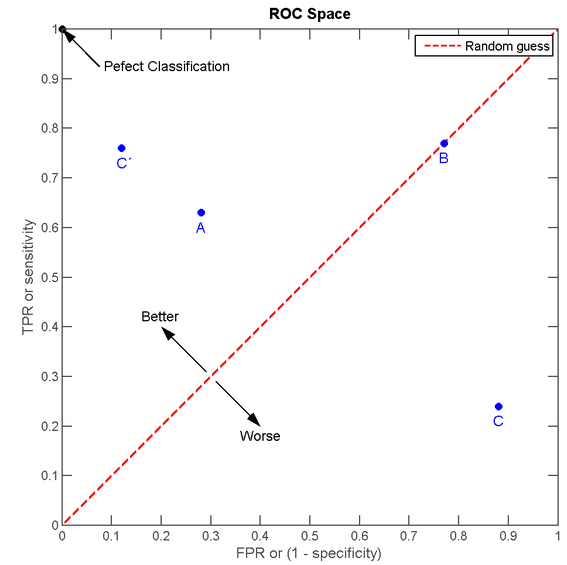
\includegraphics[width=\linewidth]{img/640px-ROC-space-2.png} 
\end{center}



ROC curves on the X-axis show a classifier's False Positive Rate so that would go from 0 to 1.0, and on the Y-axis they show a classifier's True Positive Rate so that will also go from 0 to 1.0. The ideal point in ROC space is one where the classifier achieves zero, a false positive rate of zero, and a true positive rate of one. So that would be the upper left corner. 

So curves in ROC space represent different tradeoffs as the decision boundary, the decision threshold is varied for the classifier. So just as in the precision recall case, as we vary decision threshold, we'll get different numbers of false positives and true positives that we can plot on a chart. 


\begin{center}
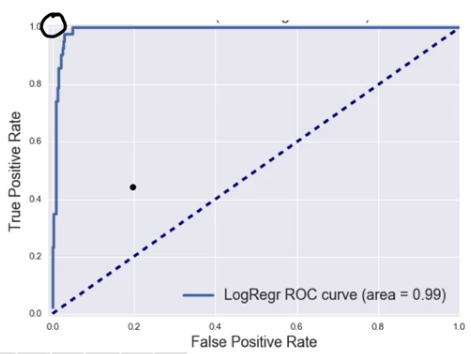
\includegraphics[width=\linewidth]{img/ROC-curve.png} 
\end{center}

The dotted line here that I'm showing is the classifier curve that secretly results from a classifier that randomly guesses the label for a binary class. 

It's basically like flipping a coin. If you have two classes with equal numbers of positive and negative incidences, then flipping a coin will get you randomly equal numbers of false positives and true positives for a large virus data sets. So the dotted line here is used as a base line. So bad classifier will have performance that is random or maybe even worse than random or be slightly better than random. Reasonably good classifier will give an ROC curve that is consistently better than random across all decision threshold choices. 

And then an excellent classifier would be one like I've shown here, which is way up into the left. 

This particular example is an example of a logistic regression classifier using the notebook example you've seen. 

So, the shape of the curve can be important as well, the steepness of the curve, we want classifiers that maximize the true positive rate while minimizing the false positive rate. 

Now as we'll see next, we can qualify the goodness of a classifier in some sense by looking at how much area there is underneath the curve. 

So the area underneath the random classifier is going to be 0.5 but then the area, as you can see, the size of the bumpiness of the classifier as it approaches the top left corner. Well, the area underneath the curve will get larger and larger. It will approach 1. And so, as we'll see in the next slide. 

\subsection{Area Under the ROC Curve (AUC)}

We use something called area under the curve, AUC. That's the single number that measures this total area underneath the ROC curve as a way to summarize a classifier's performance. So, an AUC of zero represents a very bad classifier, and an AUC of one will represent an optimal classifier. In \texttt{Scikit-learn} it is the \texttt{roc_auc_score()}.

\end{multicols}